\documentclass{beamer}
\usepackage[T1]{fontenc}
\usepackage[utf8]{inputenc}
\usepackage[italian]{babel}
\usepackage{array} % needed for \arraybackslash
\usepackage{graphicx}
\usepackage{adjustbox} % for \adjincludegraphics
\usepackage{soul}
\usepackage{color}

\usepackage{../Manoscritto/Styles/commands}

\newcommand{\nota}[1]{\textcolor{red}{#1}}

\title[]{Tensor Train Decomposition:\\ a tensor representation format for high-dimensional problems}
\author{Tommaso Bianucci}
\date{9 Giugno 2017}
\institute{Università di Pisa}
%\logo{\includegraphics[width=15mm]{logo}}
\usetheme{Dresden}
%\usecolortheme{wolverine}
%\useoutertheme[right]{sidebar}
\setbeamercovered{dynamic}
\theoremstyle{definition}
\newtheorem{definizione}{Definizione}
\theoremstyle{plain}
\newtheorem{teorema}{Teorema}

\begin{document}

\begin{frame}
\maketitle
\end{frame}

\section{Tensori}
\begin{frame}
\frametitle{Cosa sono i Tensori?}
\begin{itemize}
\item Array multidimensionali
\item Generalizzazione di vettori e matrici
\end{itemize}
\vspace{3mm}
\begin{center}
	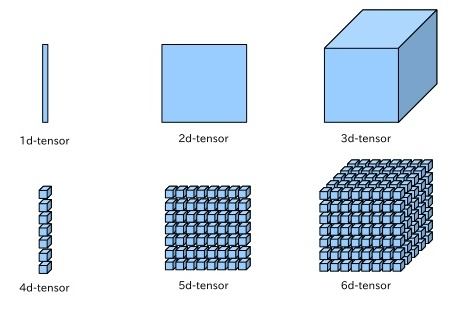
\includegraphics[width=.5\textwidth]{Img/tensors.jpg}
\end{center}
\end{frame}

\begin{frame}
\frametitle{Interesse e applicazioni}
I tensori trovano applicazione in contesti ad elevata dimensionalita', come:
\begin{itemize}
\item Deep Learning
\item Chimica computazionale
\item Analisi di segnali
\item PDE \nota{Vedi come mettere, tipo "Integrazione di PDE"}
\end{itemize}
\end{frame}

\begin{frame}
\frametitle{Tensors are hard}
I tensori sono ingombranti: $n \times n \times \cdots \times n \rightarrow n^d$
\begin{itemize}
\item Aumento esponenziale della memoria rispetto alla dimensionalita'
\item Raggiungiamo facilmente i limiti fisici del calcolatore
\end{itemize}

\vspace{5mm}

$\longrightarrow$ \emph{Curse of dimensionality}

% \vspace{5mm}

% Per poter gestire computazionalmente i tensori in modo efficace servono metodi solidi di approssimazione.
\end{frame}	

\subsection{Definizioni e strumenti}
\begin{frame}
\frametitle{Definizioni e strumenti}
\begin{itemize}
\item \nota{Fibre e fette}
\item Unfolding
\item Rango
\end{itemize}
\end{frame}

\begin{frame}
\frametitle{Unfolding}
\emph{Unfolding} o \emph{matricizzazione} e' il processo di riportare gli elementi di un tensore su una matrice.

\begin{center}
	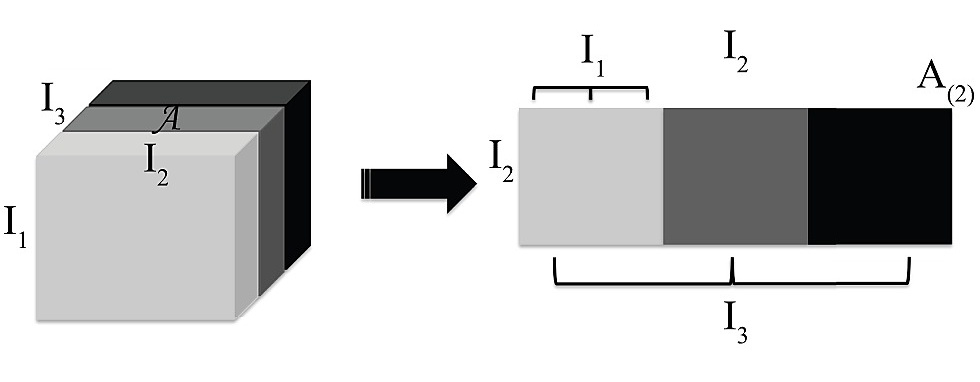
\includegraphics[width=0.5\textwidth]{Img/unfolding.jpg}
\end{center}

Preso un tensore \A, il $k$-esimo unfolding e' dato dal considerare i primi k indici e i restanti come due multi-indici:
\begin{equation*}
	A_k = A_k(
	\underbrace{I}_{i_1,\dots,i_k}
	,
	\underbrace{J}_{i_{k+1},\dots,i_d}
	) = A(i_1,\dots,i_d)	
\end{equation*}
\end{frame}

\begin{frame}
\frametitle{Rango}
Il \emph{rango} di un tensore e' il minimo numero di tensori di rango $1$ la cui somma da' il tensore di partenza.

\vspace{5mm}
Un $d$-tensore di \emph{rango} $1$ e' il risultato del prodotto esterno di $d$ vettori:

\begin{columns}
\begin{column}{0.5\textwidth}
\begin{equation*}
  \A = v^{(1)} \circ v^{(2)} \circ \cdots \circ v^{(d)}
\end{equation*}

\begin{equation*}
  a_{i_1,i_2,\ldots,i_d} = v_{i_1}^{(1)} v_{i_2}^{(2)} \cdots v_{i_d}^{(d)}
\end{equation*}
\end{column}

\begin{column}{0.5\textwidth}
\begin{center}
	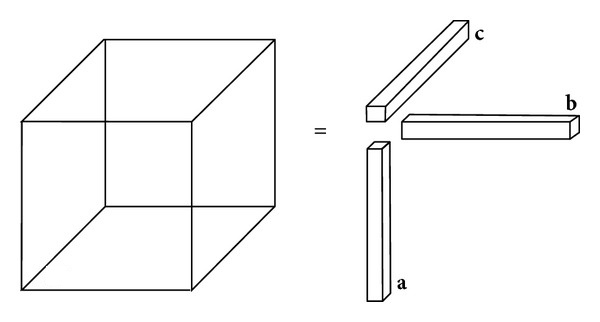
\includegraphics[width=0.8\textwidth]{Img/rank_one_tensor.jpg}
\end{center}
\end{column}
\end{columns}
\end{frame}

% \begin{frame}
% \frametitle{Problemi}
% \begin{itemize}
% \item Curse of dimensionality
% \item Determinazione del rango
% \item Degenerazione
% \end{itemize}
% \end{frame}

\subsection{Decomposizioni}
\begin{frame}
\frametitle{Decomposizioni di tensori}
Storicamente le decomposizioni principali presentate sono state: 

\vspace{5mm}
\begin{columns}
\begin{column}{0.6\textwidth}
\begin{itemize}
\item CANDECOMP/PARAFAC (CP) %\\
	% $\A \approx \sum_{r = 1}^R a_r^{(1)} \circ a_r^{(2)} \circ \cdots \circ a_r^{(d)}$
	\vspace{3mm}
\item Tucker
\end{itemize}
\end{column}
\begin{column}{0.4\textwidth}
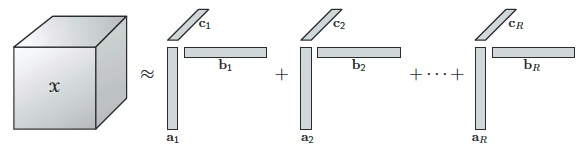
\includegraphics[width=0.85\textwidth]{Img/cp.jpg}

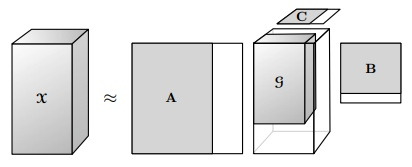
\includegraphics[width=0.7\textwidth]{Img/tucker.jpg}
\end{column}
\end{columns}

\vspace{5mm}
Teoricamente valide, ma computazionalmente problematiche:
\begin{itemize}
	\item Mancanza di algoritmi di decomposizione stabili.
	\item Dipendenza esponenziale del numero di parametri rispetto alla dimensionalita' del tensore.
\end{itemize}
\end{frame}

\section{Tensor Train}
\begin{frame}
\frametitle{Una decomposizione migliore e' possibile?}
Vorremmo una decomposizione computazionalmente maneggevole:
\begin{itemize}
\item La memoria occupata non deve dipendere esponenzialmente dal grado del tensore (fissato l'errore)
\item Deve avere un algoritmo di approssimazione e decomposizione stabile
\item Necessario poter eseguire le operazioni di algebra lineare di base direttamente nel formato \emph{compresso}
\end{itemize}
\end{frame}

\begin{frame}
\frametitle{Tensor Train Decomposition (TT)}
$\A$ tensore $d$-dimensionale, $\G_i$ \emph{core} $3$-dimensionali:
\begin{equation*}
	\A = \G_1 \G_2 \cdots \G_d
\end{equation*}
Otteniamo ogni elemento del tensore tramite moltiplicazione delle matrici $G_k(i_k)$\,:
\begin{equation*}
	\A(i_1,i_2,\dots,i_d) = 
	\underbrace{G_1(i_1)}_{1 \times r_1}
	\underbrace{G_2(i_2)}_{r_1 \times r_2}
	\cdots
	\underbrace{G_d(i_d)}_{r_{d-1} \times 1}
\end{equation*}

% \begin{center}
% 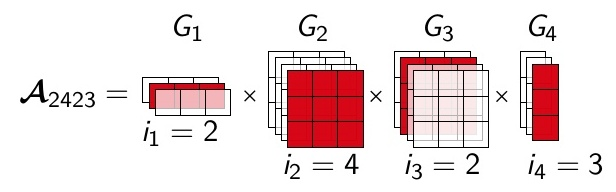
\includegraphics[width=0.5\textwidth]{Img/tt_example.jpg}
% \end{center}
Ad esempio: $\A(2,4,2,3) = \raisebox{-0.5\height}{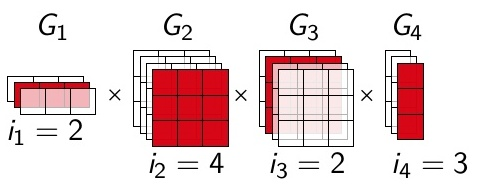
\includegraphics[width=0.4\textwidth]{Img/tt_example_2.jpg}}$
\end{frame}

\subsection{Calcolo}
\begin{frame}
\frametitle{Come calcolare la TT?}
%Abbiamo alcuni risultati:
\begin{teorema}
Sia \A un $d$-tensore e sia, per ogni $k$, $A_k$ il $k$-esimo unfolding.
Allora esiste una decomposizione TT con ranghi $r_k^{(tt)}$ t.c. $r_k^{(tt)} \leq rk(A_k) \, \forall k$
\end{teorema}

\vspace{5mm}
La dimostrazione di questo teorema:
\begin{itemize}
	\item e' costruttiva
	\item ci fornisce l'algoritmo \emph{TT-SVD}
	\item si basa sull'approssimazione delle matrici di unfolding
\end{itemize}

\nota{Metti reference a Oseledets}
\end{frame}

\begin{frame}
\frametitle{Come calcolare la TT? (2)}
\begin{teorema}
Poniamo che gli unfolding $A_k$ di \A abbiano $\epsilon$-rango $r_k$.
Allora l'algoritmo TT-SVD produce un tensore \B in formato TT, con ranghi $r_k$ e t.c. 
\begin{equation*}
    ||\A - \B ||_F \le \epsilon \sqrt{d-1}\, .
\end{equation*}

\nota{Metti reference a Oseledets}
\end{teorema}

\vspace{5mm}
Questo risultato:
\begin{itemize}
	\item assicura la stabilita' dell'algoritmo TT-SVD
	\item fornisce la soglia di approssimazione sulle SVD per ottenere la precisione desiderata sulla TT
\end{itemize}
\end{frame}

\begin{frame}
\frametitle{TT-SVD in pillole}
\nota{Inserisci qui uno schema di base dell'algo TT-SVD}
\end{frame}

\subsection{Operazioni in TT}
\begin{frame}
\frametitle{Operazioni e rounding in TT}
Molte operazioni di algebra lineare sono facilmente calcolabili direttamente in formato TT:
\begin{itemize}
\item Item 1
\item Item 2
\end{itemize}
\end{frame}

\begin{frame}
\frametitle{Quanto spazio?}
\begin{equation*}
	TT_\epsilon(\A) = 
	\underbrace{\G_1}_{1 \times n_1 \times r_1}
	\times \cdots \times
	\underbrace{\G_k}_{r_{k-1} \times n_k \times r_k}
	\times \cdots \times 
	\underbrace{\G_d}_{r_{d-1} \times n_d \times 1}
\end{equation*}	

\vspace{5mm}
Se poniamo $\,r_k \leq r\,$ e $\,n_k \leq n\,$ per $\,k = 1,\ldots,d\,$, il numero di parametri e' maggiorato da
\begin{equation*}
	2nr + (d-2)nr^2
\end{equation*}

Quindi:
\begin{itemize}
	\item non c'e' dipendenza esponenziale dall'ordine del tensore
	\item lo spazio occupato dipende molto dalla precisione scelta
\end{itemize}
\end{frame}

\subsection{In sintesi}
\begin{frame}
\frametitle{Abbiamo raggiunto i nostri obiettivi?}
\begin{itemize}
\item La memoria occupata non dipende esponenzialmente dal grado del tensore $\rightarrow$ {$\color{blue} 2nr + (d-2)nr^2$} \color{black}
\item Esiste algoritmo di approssimazione e decomposizione stabile $\rightarrow$ \textcolor{blue}{Teorema 1 + Teorema 2}
\item E' possibile eseguire le operazioni di algebra lineare di base direttamente nel formato \emph{compresso}
\end{itemize}
\end{frame}

\begin{frame}
\frametitle{Title}
\begin{itemize}
\item Item 1
\item Item 2
\end{itemize}
\end{frame}

\section{TT-Cross}
\begin{frame}
\frametitle{Title}
\begin{itemize}
\item Item 1
\item Item 2
\end{itemize}
\end{frame}

\section{Esempio}
\begin{frame}
\frametitle{Title}
\begin{itemize}
\item Item 1
\item Item 2
\end{itemize}
\end{frame}

\begin{frame}
\frametitle{Conclusioni}
I tensori sono oggetti che ci permettono di trattare problemi multidimensionali.

La TT ci permette di rendere computazionalmente accessibili questi problemi.
In particolare, in scenari di elevata dimensionalita', il procedimento di TT-CROSS rende possibile trattare problemi prima impensabili.
\end{frame}

\end{document}
